\documentclass[11pt]{article}

\usepackage[review]{acl}
\usepackage{times}
\usepackage{latexsym}
\usepackage[T1]{fontenc}
\usepackage[utf8]{inputenc}
\usepackage{microtype}
\usepackage{inconsolata}
\usepackage{graphicx}
\graphicspath{{figures/}}
\usepackage{amsmath}
\usepackage{amssymb}
\usepackage{booktabs}
\usepackage{multirow}

\title{The Temporal Tug-of-War: Visualizing and Detecting RAG Conflicts in Diffusion Models via Trajectory Variance}

\author{
  Anonymous Author(s) \\
  Affiliation \\
  \texttt{email@domain.edu}
}

\begin{document}
\maketitle

\begin{abstract}
Retrieval-Augmented Generation (RAG) introduces a failure mode in Discrete Diffusion Language Models (DLMs): when a retrieved context contradicts the model's parametric memory, the iterative denoising process becomes an observable battleground between competing knowledge sources. We propose the \textbf{Trajectory Variance Score (TVS)}, a simple and interpretable method for detecting these RAG conflicts. By computing the mean pairwise cosine distance of answer embeddings across independent stochastic denoising trajectories, TVS captures the temporal ``tug-of-war'' between parametric and contextual attractors. Our method is computationally lightweight, requiring only $N=2$ parallel inference runs. Furthermore, we demonstrate that a basic Logistic Regression classifier achieves competitive conflict detection accuracy without requiring complex sequential modeling. Finally, the TVS curve allows for easy visualization of these internal conflict dynamics across four diverse datasets (Synthetic, SciQ, PopQA, CounterFact) on LLaDA.
\end{abstract}

\section{Introduction}
The adoption of Retrieval-Augmented Generation (RAG) \citep{lewis2020retrieval} has become the standard mechanism for mitigating hallucinations in large language models. However, this architecture introduces a secondary failure mode: knowledge conflict. When an injected RAG context directly contradicts the model's pre-trained parametric memory (e.g., outdated facts or adversarially generated fakes), the model must implicitly arbitrate between its internal prior and the external evidence. 

In standard autoregressive (AR) models, this friction is instantaneous and localized, manifesting as spikes in token-level perplexity during left-to-right decoding. However, the emergence of Discrete Diffusion Language Models (DLMs) like LLaDA \citep{nie2024llada} fundamentally alters this paradigm. Unlike AR models, DLMs generate text through an iterative, non-causal denoising process. The resolution of knowledge conflicts is therefore not a single token-emission event, but a temporal "tug-of-war" distributed across the entire diffusion trajectory. 

Recent work in DLM interpretability, such as TraceDet \citep{tracedet2025}, has demonstrated that features extracted from hidden trajectories can classify intrinsic hallucinations. Building on this view, we introduce the \textbf{Trajectory Variance Score (TVS)}. We hypothesize that forced arbitration between contradictory memory sources induces measurable instability in the intermediate denoising states—and that this instability is directly observable as elevated cross-seed semantic divergence. By executing $N$ independent stochastic denoising runs and computing mean pairwise cosine distance across seed predictions at each timestep, we obtain a temporal feature vector that is both interpretable and classifiable by simple models.

Our contributions are:
\begin{enumerate}
    \item We formally define the problem of RAG-induced knowledge friction in the discrete diffusion paradigm.
    \item We propose \textbf{TVS}, computed as the mean pairwise cosine distance of sentence-embedded predictions across $N$ seeds at each denoising timestep, providing an interpretable, logit-free measure of cross-seed semantic divergence over the stochastic trajectory.
    \item We demonstrate that the TVS signal does not require complex sequential modeling: a simple Logistic Regression classifier over the flattened $T$-dimensional TVS vector achieves competitive conflict detection accuracy, matching the performance of recurrent architectures.
\end{enumerate}

\section{Related Work}

\subsection{Hallucination and Conflict Detection in AR-LLMs}
Hallucination detection in autoregressive models has been extensively studied. Output-based detection leverages signals derived from the generated text, such as semantic entropy \citep{kuhn2023semantic} or lexical similarity. The core intuition is that hallucinated or conflicting responses are associated with lower predictive confidence. Latent-based methods instead probe the hidden representations during a single forward pass, utilizing techniques like Contrast-Consistent Search (CCS) \citep{burns2022discovering} to separate truthful from hallucinated states. However, these methods are uniquely suited to the left-to-right generation paradigm and fail to capture the multi-step refinement of diffusion models.

\subsection{Discrete Diffusion Language Models}
Discrete Diffusion Language Models have emerged as alternatives to AR models \citep{sahoo2024simple, shi2024simplified}. Models such as LLaDA \citep{nie2024llada} utilize discrete remasking processes to scale up to 8B parameters, achieving performance comparable to leading LLMs. Similarly, DREAM \citep{zheng2024dream} adapts diffusion paradigms for enhanced reasoning. Recent efforts like SPREAD \citep{spread2026} have begun exploring DLMs within the RAG framework, identifying Response Semantic Drift (RSD) and employing query-relevance-guided denoising to keep generation anchored to the query semantics. Furthermore, while recent work like Adaptive Retrieval-Augmented Masked Diffusion (ARAM) \citep{aram2026} attempts to force alignment via adaptive logit guidance, our work is fundamentally different because it provides a post-hoc interpretability window without altering the generation process. Consequently, the specific mechanisms of detecting the underlying parametric versus external knowledge conflicts remain underexplored.

\subsection{Trajectory Analysis in Diffusion Models}
The shift to iterative refinement necessitates new interpretability tools. The most relevant precursor to our work is TraceDet \citep{tracedet2025}, which formulates the denoising process as an action trace and applies the Information Bottleneck principle to extract sub-traces informative of hallucinated outputs. TDGNet \citep{tdgnet2026} learns over evolving token-level attention graphs, while OSCAR \citep{oscar2026} computes cross-chain Shannon entropy across parallel denoising chains with randomized reveal orders to detect high-uncertainty token positions. While OSCAR and TVS both exploit parallel denoising runs, they differ fundamentally: OSCAR operates token-by-token within a single pass to flag high-entropy positions; TVS measures the \textit{temporal evolution of cross-run semantic divergence} in the answer entity embedding space—a complementary signal that captures how competing knowledge sources destabilize generation dynamics over the full denoising schedule. None of these methods address the specific phenomenon of RAG-induced knowledge friction, nor demonstrate that the resulting signal can be classified without complex sequential modeling.

\section{Background: Diffusion Large Language Models}

\subsection{Formal Formulation of D-LLMs}
Unlike AR models that rely on the next-token prediction paradigm $P(x_i | x_{<i})$, DLMs generate responses by iterative refinement through a forward noising and backward denoising process over $T$ time steps. 

Let $r = (r_0, \dots, r_T)$ denote the sequence of intermediate texts, where each $r_t \in \mathcal{V}^n$ is a token sequence of length $n$. Here, $r_0$ represents the fully clean, structured text sequence, and $r_T$ represents the fully masked sequence (pure noise). 

Given an input query $p_0$, the \textbf{forward noising process} is defined by a sequence of transition distributions $\{q(r_t | r_{t-1})\}_{t=1}^T$, mathematically expressed as:
\begin{equation}
    q(r_{1:T} | r_0) = \prod_{t=1}^T q(r_t | r_{t-1})
\end{equation}
This process gradually corrupts the sequence by replacing tokens with a designated `[MASK]` state.

Conversely, the \textbf{reverse denoising process} is parameterized by a neural network defining a sequence of conditional distributions $\{P_\theta(r_0 | r_t, p_0)\}_{t=1}^T$. At each timestep $t > 0$, the model predicts all masked tokens simultaneously from the current state $r_t$, yielding an estimated clean sequence $\tilde{r}_{t-1} \sim P_\theta(r_0 | r_t, p_0)$. Following this prediction, a discrete remasking strategy is applied (typically low-confidence remasking) where a specific fraction $\rho_t$ of the predicted tokens are remasked to form the intermediate state $r_{t-1}$.

\subsection{Knowledge Friction in the Denoising Trajectory}
We model the generation process as a stochastic denoising trajectory $\tau = (r_0, r_1, \dots, r_T)$, where each intermediate state $r_t$ represents a partially-unmasked sequence. Under a clean RAG context, the trajectory converges smoothly toward a single semantic attractor. Under a conflicting context, competing knowledge sources (the parametric prior $\theta_{true}$ and the injected context $p_0$) create sustained instability in the intermediate states, a phenomenon we term \textbf{Knowledge Friction} \citep{spread2026}.

For example, given the query \textit{``What is the capital of France?''} the model's prior strongly associates the answer with \textit{``Paris''} ($\theta_{true}$). If the injected RAG context states \textit{``The capital of France is London''} ($p_0$), the stochastic denoising trajectory oscillates between these competing attractors before crystallizing. Because DLMs decode all positions in parallel, this friction is distributed globally across the full denoising schedule rather than localized to a single token emission event.

\section{Methodology: Trajectory Variance Score}

To detect this knowledge friction, we isolate the temporal instability it creates by measuring the semantic divergence across multiple independent stochastic denoising runs. The end-to-end pipeline is illustrated in Figure~\ref{fig:pipeline}.

\begin{figure}[h]
\centering
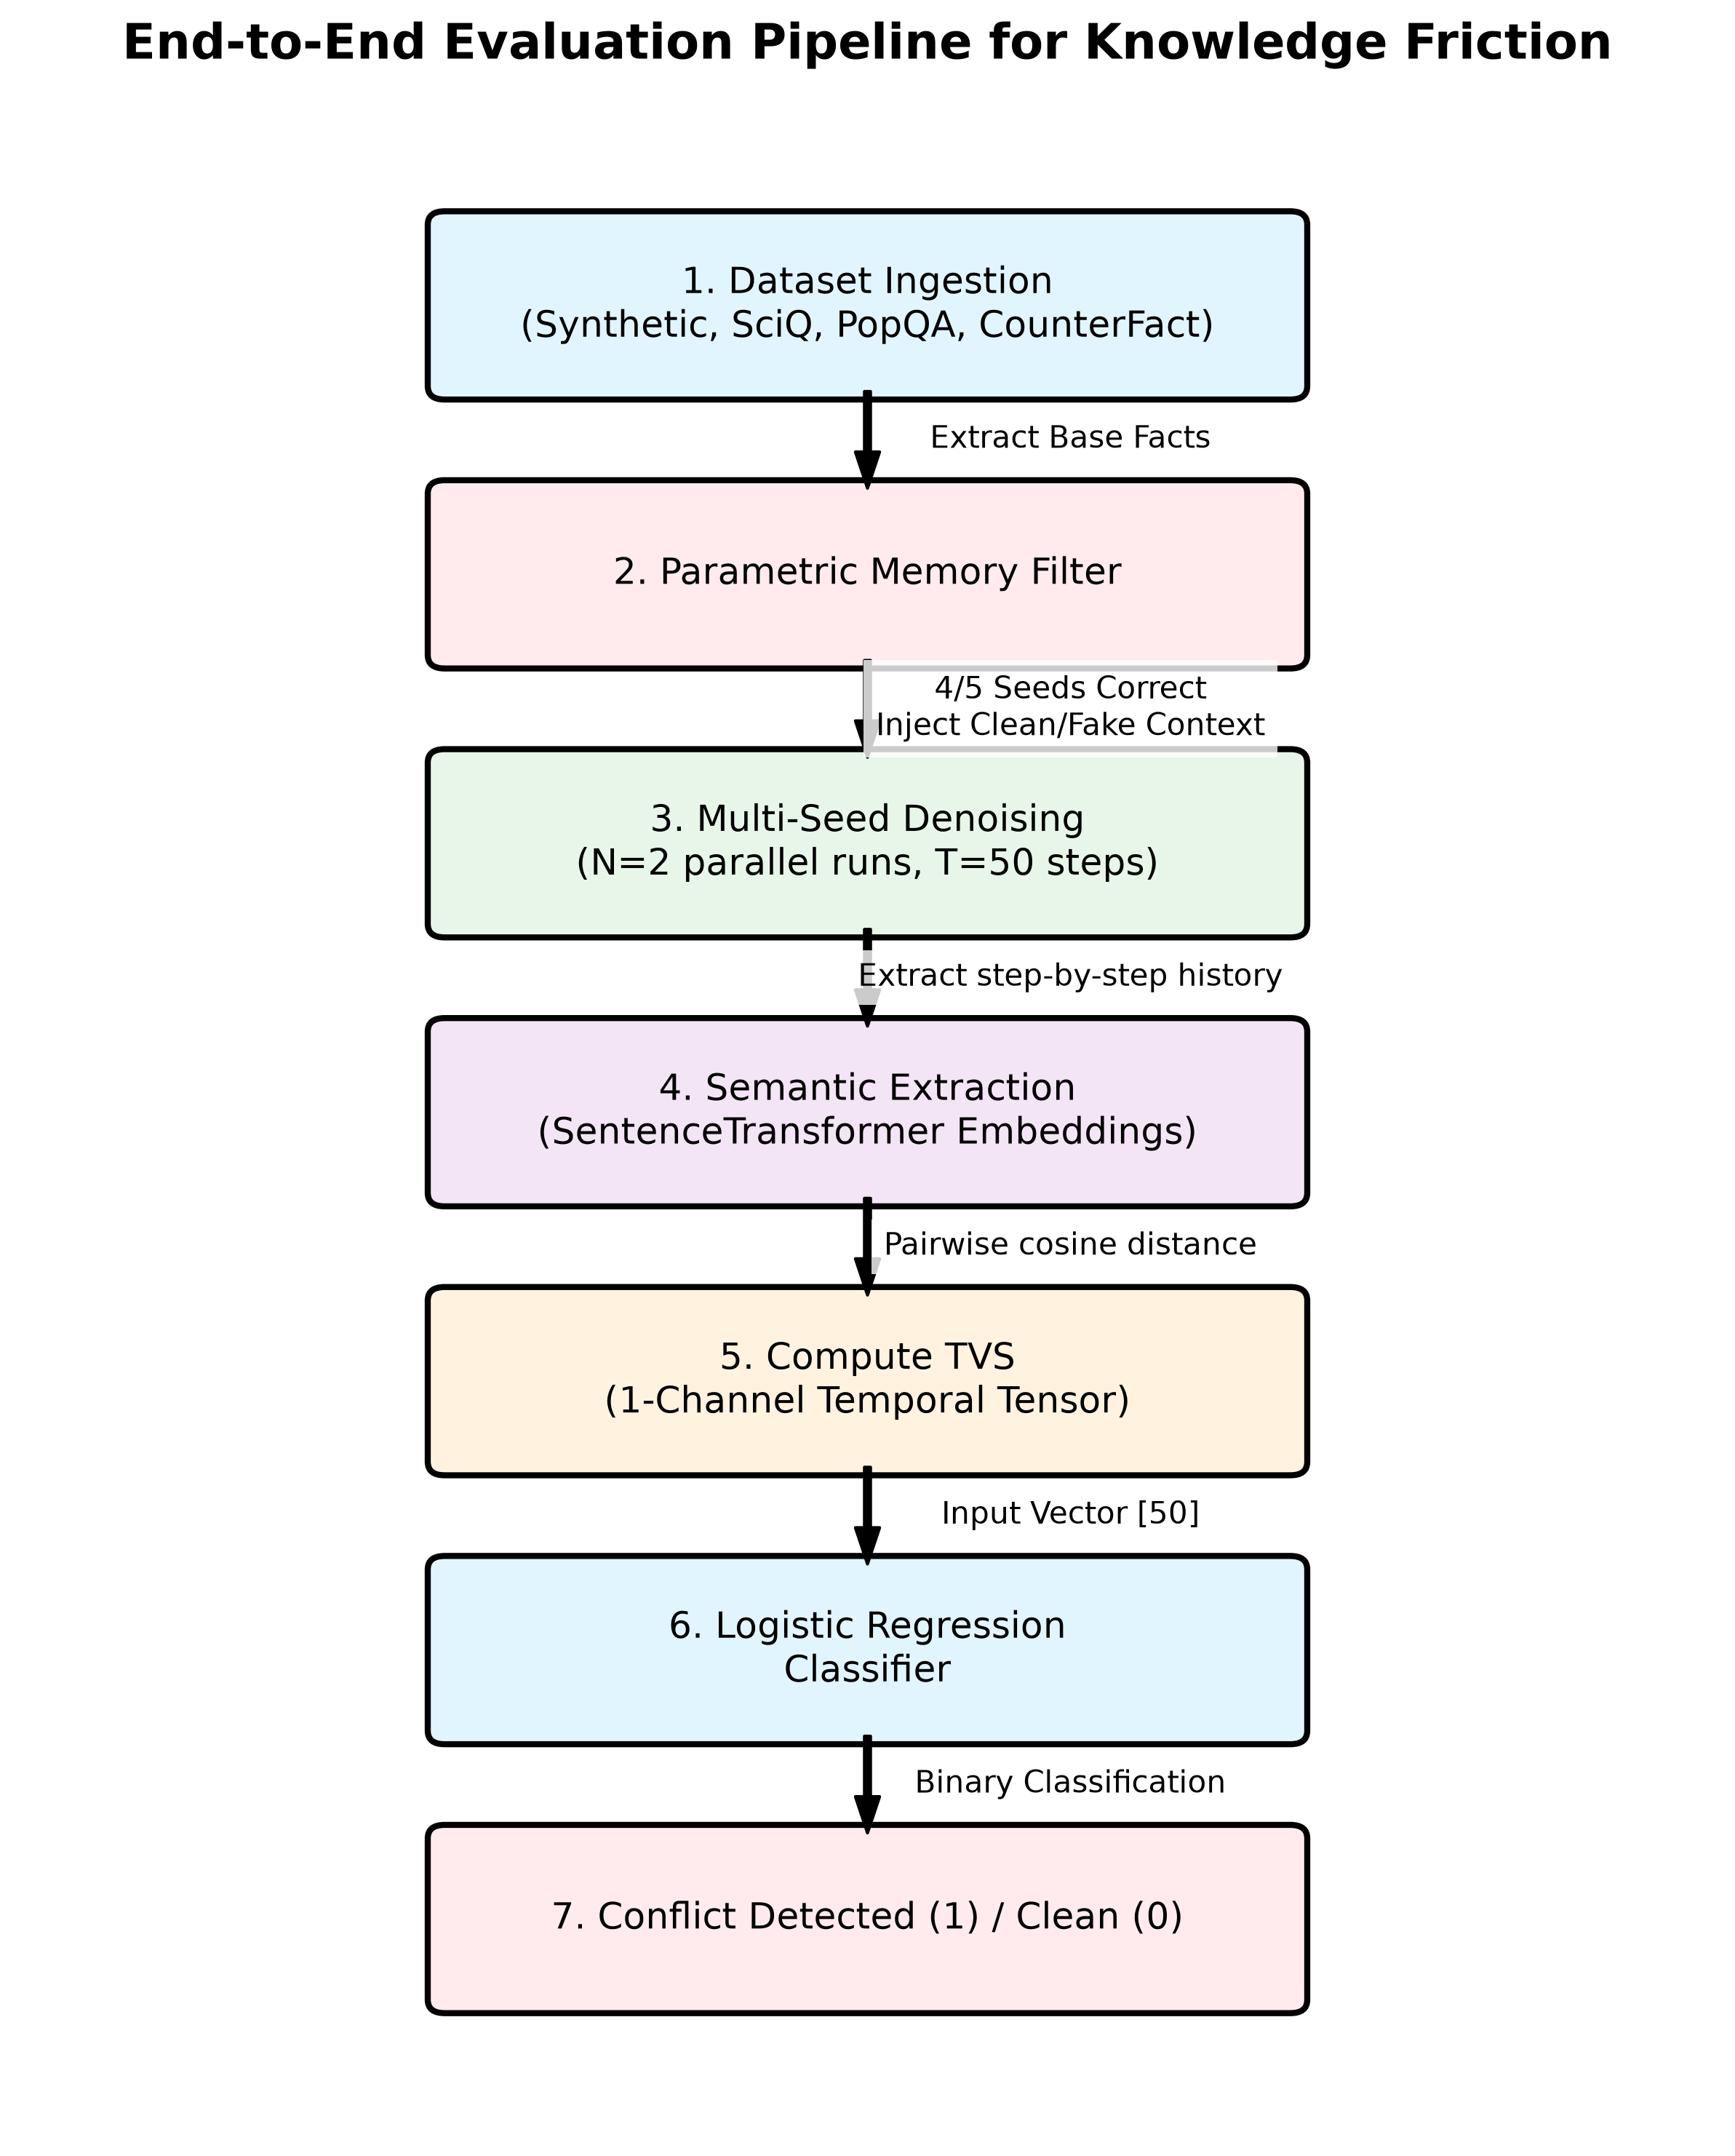
\includegraphics[width=\columnwidth]{pipeline.png}
\caption{End-to-end evaluation pipeline: facts undergo parametric memory filtering, conflict contexts are injected, $N=2$ independent denoising trajectories are executed, the mean pairwise cosine distance (TVS) is computed at each of $T=50$ timesteps, producing a $T$-dimensional feature vector, and the resulting vector is classified by a Logistic Regression detector.}
\label{fig:pipeline}
\end{figure}

\subsection{Parametric Memory Filtering and Trajectory Generation}
Diffusion models are inherently stochastic; each denoising trajectory depends on the initial random seed governing the remasking schedule. Before generating conflict trajectories, we apply a rigorous parametric memory filter: a fact is retained only if the base DLM correctly generates the true answer across at least 4 out of $N=5$ independent seeds. This ensures subsequent friction is genuinely induced by the RAG context rather than inherent model ignorance. After filtering, \textbf{2,947 facts} survived for LLaDA evaluation (yielding 5,894 balanced clean/conflict sample pairs).

For each verified fact, we execute $N=2$--$5$ independent stochastic denoising runs over $T=50$ diffusion timesteps. At each run $i$ and timestep $t$, we decode the model's predicted token sequence. We isolate the answer entity from the full generation via exact sub-string matching against the target, and embed it using the \texttt{all-mpnet-base-v2} sentence encoder to obtain embedding $\mathbf{e}_{i,t} \in \mathbb{R}^d$.

\subsection{TVS Formulation}
In the absence of knowledge friction, all $N$ runs rapidly converge on identical semantic structures, yielding low cross-seed divergence. Under conflict, competing knowledge sources cause the denoising trajectories to diverge before finally crystallizing.

At each timestep $t$, we isolate the predicted answer entity from each seed's decoded text, embed it using a frozen sentence encoder, and compute the mean pairwise cosine distance across the $N$ seed embeddings:
\begin{equation}
  \text{TVS}_t = \frac{1}{\binom{N}{2}} \sum_{i < j} \left(1 - \cos(\mathbf{e}_{i,t},\, \mathbf{e}_{j,t})\right)
\end{equation}
where $\mathbf{e}_{i,t} \in \mathbb{R}^d$ is the sentence embedding of the predicted entity at seed $i$, timestep $t$, and $\cos(\cdot,\cdot)$ denotes cosine similarity. This formulation directly measures semantic divergence in embedding space, making it interpretable and independent of the model's internal logits.

This yields a feature vector $\mathbf{v} = [\text{TVS}_1, \dots, \text{TVS}_{50}] \in \mathbb{R}^{T}$, one scalar per timestep, directly capturing how cross-seed semantic divergence evolves over the denoising schedule.

\subsection{Classification via Logistic Regression}
We classify the TVS feature vector using a \textbf{Logistic Regression} model (\texttt{max\_iter=2000}, $\ell_2$ regularization). This linear model achieves competitive accuracy, confirming the conflict signal is globally distributed across the dispersion curve.

\section{Experimental Setup}

\subsection{Models and Datasets}
We evaluate TVS on \textbf{LLaDA} \citep{nie2024llada}. Our testbed comprises four datasets: \textbf{Synthetic} (custom queries generated via LLM templates to explicitly pair simple facts with direct contradictions), \textbf{SciQ} \citep{welbl2017crowdsourcing}, \textbf{PopQA} \citep{mallen2023entity}, and \textbf{CounterFact} \citep{meng2022locating}. We selected these because their factual format enables straightforward injection of contradictory information. We randomly select 3,000 instances per dataset. We filter these for instances where the base DLM correctly generates the true answer purely from parametric memory across $\geq 4/5$ seeds. This strict parametric filter heavily decimates datasets with lower baseline knowledge: of the 12,000 initial candidates, only \textbf{2,947 facts} survived for LLaDA (SciQ: 1,448; CounterFact: 870; Synthetic: 364; PopQA: 265). To simulate conflict, we inject a contradictory RAG context, yielding 5,894 balanced paired samples. The final dataset is pooled across all domains and uses a 70/15/15 stratified train/validation/test split.

\subsection{Implementation Details}
Trajectories were collected using $N=2$ to $5$ seeds over $T=50$ timesteps. Sentence embeddings use the frozen \texttt{all-mpnet-base-v2} model. The Logistic Regression is trained on the pooled, flattened $\mathbf{v} \in \mathbb{R}^{50}$ TVS feature vectors (\texttt{max\_iter=2000}, $\ell_2$ regularization). All results are reported as mean $\pm$ standard deviation over 5 independent random train/test splits.

\section{Results}

\subsection{Overall Detection Performance}
Table~\ref{tab:overall_results} presents the overall conflict detection performance of our TVS approach. As an informal point of reference, we also include a best-effort replication of TraceDet's Variational Information Bottleneck trajectory classifier (the original codebase is not publicly available and has not been formally verified on this task). Our simple linear TVS classifier achieves $70.76\% \pm 0.62\%$ accuracy, performing similarly to this approximated baseline. This demonstrates that TVS provides a viable and highly interpretable embedding-based feature space without requiring opaque sequential modeling.

\begin{table}[h]
\centering
\resizebox{\columnwidth}{!}{%
\begin{tabular}{lcc}
\toprule
\textbf{Method} & \textbf{Acc (\%)} & \textbf{AUROC} \\
\midrule
TraceDet* & $71.34 \pm 0.66$ & $0.7865 \pm 0.0078$ \\
TVS-LR (Ours) & $70.76 \pm 0.62$ & $0.7725 \pm 0.0082$ \\
\bottomrule
\end{tabular}%
}
\caption{Overall conflict detection performance (LLaDA, mean $\pm$ std over 5 random splits). TVS achieves competitive accuracy while using an interpretable, embedding-based feature space. *TraceDet codebase is not publicly available; we benchmark against an unverified best-effort replication for context.}
\label{tab:overall_results}
\end{table}

\begin{table}[h]
\centering
\resizebox{0.6\columnwidth}{!}{%
\begin{tabular}{lc}
\toprule
\textbf{Metric} & \textbf{Score (\%)} \\
\midrule
Precision & $72.95 \pm 1.32$ \\
Recall & $66.05 \pm 1.46$ \\
F1-Score & $69.30 \pm 0.60$ \\
\bottomrule
\end{tabular}%
}
\caption{Classification metrics for Logistic Regression (LLaDA, mean $\pm$ std over 5 random splits).}
\label{tab:classification_report}
\end{table}

\subsection{Dataset-Specific Dynamics}
Table~\ref{tab:dataset_breakdown} provides the per-domain accuracy breakdown (LR classifier, averaged over 5 random splits).

\begin{table}[h]
\centering
\resizebox{\columnwidth}{!}{%
\begin{tabular}{cccc}
\toprule
\textbf{Synth.} & \textbf{SciQ} & \textbf{PopQA} & \textbf{CounterFact} \\
\midrule
$77.31 \pm 5.92$ & $74.52 \pm 1.44$ & $72.34 \pm 1.35$ & $61.80 \pm 2.48$ \\
\bottomrule
\end{tabular}%
}
\caption{Detection accuracy (\%) by domain (LLaDA, LR classifier, mean $\pm$ std over 5 splits). CounterFact is consistently the hardest domain ($61.80\%$), suggesting counterfactual injections trigger rapid parametric override with less sustained trajectory friction.}
\label{tab:dataset_breakdown}
\end{table}

The model performs best on Synthetic facts ($\sim$77.3\%) and worst on CounterFact ($\sim$61.8\%). The high performance on the Synthetic dataset is likely an artifact of its templated construction: because the injected conflicts are structurally uniform, they produce an exceptionally clean and distinguishable friction signal compared to the noisier, natural phrasing in PopQA or SciQ. Furthermore, because the rigorous 4-of-5 parametric filter disproportionately decimates CounterFact (870 facts) and PopQA (265 facts) relative to their initial 3,000-sample pools, these lower accuracies are harder to interpret and may reflect the skewed distribution of the pooled training set rather than inherent dataset difficulty. Furthermore, the CounterFact difficulty likely arises because semantically extreme counterfactuals (e.g., ``The capital of France is London'') override the parametric prior so decisively that cross-seed divergence collapses early, leaving a weak TVS signal.

\section{Ablation Studies}
\label{sec:ablation}

\subsection{Architecture Comparison: Is Sequential Modeling Required?}
Table~\ref{tab:ablation_arch} compares three classifier architectures over 5 random splits on the TVS feature vector.

\begin{table}[h]
\centering
\resizebox{\columnwidth}{!}{%
\begin{tabular}{lcc}
\toprule
\textbf{Classifier} & \textbf{LLaDA Acc (\%)} & \textbf{LLaDA AUROC} \\
\midrule
Logistic Regression & $71.05 \pm 0.72$ & $0.7701 \pm 0.0098$ \\
LSTM (Uni-directional) & $71.75 \pm 0.54$ & $0.7895 \pm 0.0061$ \\
Bi-LSTM + Attention & $71.93 \pm 0.71$ & $0.7906 \pm 0.0062$ \\
\bottomrule
\end{tabular}%
}
\caption{Architecture comparison over 5 random splits (LLaDA). All confidence intervals overlap substantially. The Bi-LSTM is only $0.88\%$ more accurate than a simple Logistic Regression.}
\label{tab:ablation_arch}
\end{table}

The marginal performance gap between the simple linear model and the complex recurrent architectures suggests that the classifier is primarily exploiting the overall magnitude of dispersion rather than complex temporal dependencies. To rigorously test this, we evaluated both the Logistic Regression and the LSTM on a dataset where the 50 timestep features were randomly shuffled (consistently across all samples). By construction, the Logistic Regression's accuracy is invariant to feature permutation and remains identically unchanged. Empirically, the LSTM's accuracy also did not drop under this shuffling constraint (remaining at $\sim$70.6\%). This confirms that no sequential structure is being exploited by any model, and that recurrent architectures do not extract meaningful signal beyond what the order-invariant linear baseline already captures.


\subsection{Seed Count Ablation: How Many Runs Are Needed?}
Table~\ref{tab:ablation_seeds} evaluates the effect of reducing the number of parallel denoising runs $N$, using the Logistic Regression classifier.

\begin{table}[h]
\centering
\resizebox{\columnwidth}{!}{%
\begin{tabular}{ccc}
\toprule
\textbf{$N$ Seeds} & \textbf{LLaDA Acc (\%)} & \textbf{LLaDA AUROC} \\
\midrule
2 & $70.76 \pm 0.62$ & $0.7725 \pm 0.0082$ \\
3 & $71.75 \pm 1.06$ & $0.7806 \pm 0.0084$ \\
5 & $71.23 \pm 1.00$ & $0.7851 \pm 0.0074$ \\
\bottomrule
\end{tabular}%
}
\caption{Effect of seed count on detection performance (LLaDA, LR classifier, 5 random splits). The gap between $N=2$ and $N=5$ is within overlapping error bars, demonstrating that two parallel runs are sufficient for deployment.}
\label{tab:ablation_seeds}
\end{table}


\section{Analysis: Interpreting the Tug-of-War}
Figure~\ref{fig:avg_tvs} plots the average Cosine Dispersion (TVS) over the 50-step denoising trajectory, revealing that knowledge friction manifests as a sustained, three-phase elevation in cross-seed semantic divergence.

\begin{figure}[ht]
    \centering
    
\includegraphics[width=0.9\columnwidth]{tvs_conflict_graph.png}
    \caption{Average Cosine Dispersion (TVS) across the 50-step denoising trajectory for LLaDA (Clean: blue solid; RAG Conflict: red dashed; shaded = SEM). Three phases are visible: \textbf{Zone 1} ($t \in [0, 15]$): Early Exploration---both conditions exhibit high dispersion as the model samples candidate answers. \textbf{Zone 2} ($t \in [15, 28]$): Mid-Step Friction---the clean curve decays as generation crystallizes around the context-aligned answer, while the conflict curve remains elevated (gap $\approx 0.15$) due to competing parametric and contextual attractors. \textbf{Zone 3} ($t \in [28, 50]$): Delayed Crystallization---both curves collapse, but a residual dispersion gap persists ($\Delta \approx 0.07$), reflecting weaker semantic commitment under conflict.}
    \label{fig:avg_tvs}
\end{figure}

\begin{figure}[ht]
    \centering
    
\includegraphics[width=\columnwidth]{tvs_raw_dynamics_with_errorbars.png}
    \caption{Detailed TVS dynamics for LLaDA with $\pm$std shading ($N=2$ seeds). The conflict curve (red) starts at $\approx 0.51$ vs.~clean (green) at $\approx 0.39$, maintaining a consistent gap through $t\approx28$ before both converge---with conflict retaining a higher residual dispersion ($\approx 0.07$ vs.\ $\approx 0.01$).}
    \label{fig:tvs_dynamics}
\end{figure}

The conflict trajectory (red dashed) starts at $\text{CD} \approx 0.51$ versus $0.39$ for clean (blue solid), maintaining a gap of $\sim$0.1--0.15 throughout Zone 1 and Zone 2. Both curves collapse rapidly after $t \approx 28$, but a residual gap of $\approx 0.07$ persists at convergence, representing the ``crystallization gap'' that distinguishes conflict samples even after generation terminates. This three-phase structure directly motivates the temporal feature representation: a simple classifier over the dispersion curve captures the sustained divergence without requiring a sequential model.

\subsection{The Value of the Temporal Trajectory}
To explicitly address whether the intermediate diffusion trajectory provides signal beyond standard output-level multi-sample variance (analogous to autoregressive semantic entropy), we evaluated a Logistic Regression trained strictly on the final crystallization step ($\text{TVS}_{50}$). This trivial baseline achieved only $60.14\% \pm 0.57\%$ accuracy. The $\sim$11\% performance drop compared to the full $T$-dimensional TVS vector ($71.05\%$) empirically proves that the mid-step ``tug-of-war'' dynamics contain critical diagnostic signal for detecting knowledge friction that is lost if one only evaluates the final generated output.

\section{Conclusion}
We introduced the Trajectory Variance Score (TVS), a simple and interpretable method for detecting RAG-induced knowledge conflicts in Discrete Diffusion Language Models. By computing mean pairwise cosine distance across $N=2$ stochastic denoising trajectories at each timestep, TVS produces a $T$-dimensional feature vector. We demonstrate that a simple Logistic Regression classifier over this vector achieves competitive detection accuracy, proving that no complex sequential modeling is required to extract the conflict signal. The TVS curve directly visualizes the temporal tug-of-war between parametric and contextual attractors as a three-phase dynamics profile. With only two parallel inference runs needed, TVS is a computationally lightweight and interpretable diagnostic for investigating knowledge friction in diffusion language models.

\section{Limitations}
TVS requires multiple parallel denoising runs, which introduces inference overhead compared to single-pass methods. Additionally, our pipeline relies on exact sub-string matching to isolate answer entities; this rigid extraction step is a potential failure point for valid paraphrases or partial matches, leading to unquantified extraction failure rates. A further limitation is that TVS relies on a parametric memory filter that itself requires $N=5$ generation runs at evaluation time; exploring lighter filtering strategies is a promising direction for future work.

\section*{Ethics Statement}
As language models are increasingly deployed in real-world applications via Retrieval-Augmented Generation, their susceptibility to knowledge conflicts poses significant risks of propagating misinformation or adversarial fakes. The Trajectory Variance Score (TVS) provides an interpretability mechanism to detect and intercept these hallucinations before they reach the end user. While TVS significantly enhances the transparency of discrete diffusion models, it should not be treated as a standalone safeguard. It is intended to complement, rather than replace, standard fact-checking pipelines, ensuring that AI systems remain trustworthy and aligned with factual reality.

\bibliography{custom}

\end{document}